%Travail technique
	%But?
	%Overview (Mockups, workflows)
	%Algorithme
	%Architecture et Design
	%Implémentation (langage et librairies utilisés)
	%Utilisation (screenshots, etc)


\chapter{Travail technique}
	\thispagestyle{document}
	
\section{Principe}
\label{sec:principe}

\par Le principe est d'utiliser les suites de tests d'un projet comme spécifications de celui-ci. Chacune d'entre elles est liée à une méthode. Lors de l'exécution des tests, toutes les variables accessibles depuis la dernière ligne de la méthode référencée seront collectées. De plus, les assertions contenu dans le test permettent de récupérer les valeurs attendu par l'exécution de la méthode ciblée, ce sont les oracles. Il est ensuite possible de combiner de nombreuse manières les valeurs collectées avec des opérateurs afin d'essayer de faire correspondre une expression avec les oracles. Si une tel combinaison existe, la dernière ligne de la méthode est donc synthétisable, sinon il faudra réitérer après avoir synthétiser d'autres lignes, modifiant ou augmentant les valeurs collectées.

\section{Hypothèses de travail}
\label{sec:hypotheses}


\par OLS-Test se limite uniquement aux méthodes ayant un type de retour, les méthodes de type \textit{void} ne peuvent pas être synthétisées. De plus, la phase de collecte des oracles ne permet pas de récupérer une sortie de type exception lorsqu'elle n'est pas spécifiée dans une assertion (\textit{@Test en java}). Lors de la synthèse, uniquement la dernière ligne de la méthode sera synthétisée, le reste de la méthode ne sera pas modifié. De part le fait que la collecte des oracles est dynamique, il n'y pas de limite sur la complexité ou l'écriture d'un test.



\section{Overview}
\label{sec:overview}

\subsection{Référencement des méthodes à synthétiser}
\label{subsec:ciblage}
\par Les méthodes testées doivent être référencés de manières explicites dans les tests associés. Une convention a été mise en place, le développeur doit ensuite la respecter lors de l'écriture des spécifications. La figure \ref{fig:ciblage} représente un exemple de référencement. À la différences des annotations, cette convention ne demande pas d'ajouter de nouvelle dépendances à un projet car elle utilise simplement la documentation.

\begin{figure}[H]
\begin{lstlisting}
/**
 * @see mon.package.MaClass#MaMethod(type.param1, type.param2)
 */
\end{lstlisting}
\caption{Exemple de référencement utilisé à l'aide de la Javadoc}
\label{fig:ciblage}
\end{figure}



\subsection{Collecte des données nécessaires}

\subsubsection{Collecte des variables accessibles depuis une position}
\label{subsec:collecte_entree}
\par La collecte des variables accessibles depuis une position est effectuée par DynaMoth. Cette position correspond à la dernière ligne de la méthode ciblée. DynaMoth utilise ensuite une API\footnote{\url{https://fr.wikipedia.org/wiki/Interface_de_programmation}} de débogage pour placer un point d'arrêt à cette position. Il collecte ensuite toutes les valeurs accessibles : les variables, les attributs et même les appels de méthodes. Des constantes peuvent également être ajoutées. La figure \ref{fig:exemple_collecte} est un exemple de collecte à partir d'une position donnée.

\begin{figure}[H]
\begin{lstlisting}
 1 public class Exemple {
 2 
 3	private int zero = 0;
 4
 5	public int addOne(int a){
 6		return a + 1;
 7	}
 8	public int max(int a, int b){
 9		if ( a > b )
10			return a;
11		return b;	
12	}
13 }
\end{lstlisting}
\begin{center}

\begin{tabular}{|c|c|c|c|}
\hline
Constante & Variable & Attribut & Méthode  \\
\hline
-1 & a & zero & addOne\\
\hline
0  & b & &\\
\hline
1  &  & & \\
 \hline
\end{tabular}

\end{center}
\label{fig:exemple_collecte}
\caption{Exemple de valeurs collectées à partir de la ligne 11}
\end{figure}

\subsubsection{Collecte des oracles lors de l'exécution des tests}
\label{subsec:collecte_sorties}
\par La collecte des oracles s'effectue en modifiant les tests et en les exécutants. La transformation représentée dans la figure \ref{fig:collect_sorties} a pour but de récupérer les valeurs attendues par les assertions pour ensuite les envoyer à DynaMoth. Les oracles sont collectés et évaluées de manières dynamiques.

\begin{figure}[H]
\begin{lstlisting}
methodTest :
+   collect(methodeCible.signature, methodTest.signature, sortie1)
    assertion(sortie1, methodeCible(param1))
+   collect(methodeCible.signature, methodTest.signature, sortie1)
    assertion(sortie2, methodeCible(param1))
\end{lstlisting}
\caption{Exemple de transformation pour récupérer les oracles}
\label{fig:collect_sorties}
\end{figure}

\subsection{Combinaison des différents opérateurs de synthèse}
\label{subsec:combinaisons}

\par Une fois les variables accessibles depuis une position donnée collectées, il faut les faire correspondre avec les oracles, pour chaque exécution de la position. Si cette correspondance n'est pas direct, DynaMoth essaye de combiner les variables avec des opérateurs pour agrandir l'ensemble des possibilités. Il recommence récursivement jusqu'à trouver une relation, ou atteindre un \textit{timeout} paramètrable. La table \ref{fig:operateurs} représente les opérateurs utilisées par DynaMoth.

\begin{table}[H]
\centering
\begin{tabular}{|c|c|}
\hline
Opérateurs & ! ++ $--$ \&\& $|$ $|$ == != $<$= $<$ + $-$ * / \% [appel de méthode]\\
\hline
\end{tabular}
\caption{Les opérateurs utilisés par DynaMoth}
\label{fig:operateurs}
\end{table}
 

\section{Implementation}
\label{sec:implementation}

\par OLS-Test est implementé en Java, pour les différentes transformation et instrumentation de code source, il utilise Spoon\footnote{\url{http://spoon.gforge.inria.fr/}}. Les spécifications sous forme de tests sont également écrite en Java, à l'aide du framework JUnit\footnote{\url{http://junit.org/}}. Comme énoncé en \ref{subsec:ciblage}, le référencement de méthode utilise la Javadoc et \textit{@see}. OLS-Test utilise également Maven Invoker API\footnote{\url{https://maven.apache.org/shared/maven-invoker/}}, afin de démarrer différent \textit{goals} sur le projets en cours d'analyse.


\subsection{Injection du harnais de test}

\par La phase de collecte des oracles expliquée en \ref{subsec:collecte_sorties} s'effectue de la manière suivante. Les tests sont modifiées à l'aide Spoon pour récupérer les valeurs attendues par les assertions. Or, puisque ces tests seront exécuter à l'aide de Maven Invoker API, le context de OLS-Test ne sera pas accessible. Pour résoudre se problème, OLS-Test injecte également un harnais de test dans le projet contenant les méthodes à synthétiser. Ce harnais est composé d'un \textit{Runner} personnalisé, ainsi que d'une structure contenant les différents oracles durant l'exécution. La collecte se fera donc dans le context du projet passé en paramètre. À la fin de l'exécution des tests, le \textit{Runner} sérialise les oracles dans un fichier. Il ne restera plus qu'à OLS-Test de les récupérer une fois le \textit{goal} maven terminé. La figure \ref{fig:workflow_collectes_sorties} représente le workflow lors de la phase de collecte des sorties.

\begin{figure}[H]
\begin{center}
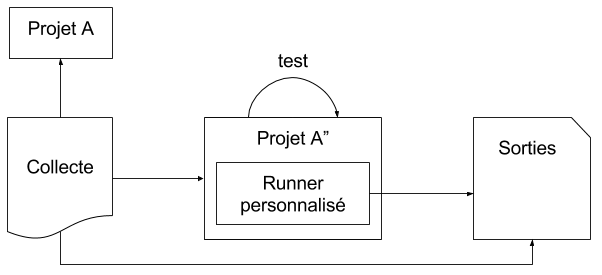
\includegraphics[scale=.7]{Workflow_output_collector.png}
\end{center}
\caption{Workflow d'exécution lors de la collecte des sorties}
\label{fig:workflow_collectes_sorties}
\end{figure}

\subsection{Conservation du comportement original des tests}

\par Le framework JUnit fonctionne le manière suivante, lors qu'une assertion échoue à l'intérieur d'un test, elle soulève une exception. Cependant, lors d'un tel comportement, les assertions suivantes ne seront pas exécutées et donc pas collectées. Afin collecter toutes les sorties, la transformation appliquée insert également des \textit{try/catch} pour ne pas stopper l'exécution du test. Une exception est soulevée à la fin du test, uniquement si l'une des assertions a échoué. La figure \ref{fig:collect_sorties_try_catch} reprend l'exemple énoncé en \ref{subsec:collecte_sorties} en appliquant cette transformation supplémentaire.

\begin{figure}[H]
\begin{lstlisting}
public void test() :
+ hasException=false
+ try
+   collect(methodeCible.signature, methodTest.signature, sortie1)
    assertion(sortie1, methodeCible(param1))
+ catch AssertionError
+   hasException=true
+ try
+   collect(methodeCible.signature, methodTest.signature, sortie2)
    assertion(sortie2, methodeCible(param1))
+ catch AssertionError
+   hasException=true
+ assertion(hasException, false)
\end{lstlisting}
\caption{Exemple de transformation spécifique à JUnit pour récupérer les oracles}
\label{fig:collect_sorties_try_catch}
\end{figure}






\section{Utilisation}

\begin{figure}[H]

\begin{verbatim}
Usage: OLS_Test
	    -s, --source-path           path_program
	    -m, --maven-home-path       path_maven_home
   [-c, --constant              one_constant_to_add]*
   [-t, --time-out-collection   time in second]
   [-d, --time-out-dynamoth     time in second]
   [-o, --override]
   [-v, --verbose]
\end{verbatim}

\end{figure}
	

	
		
		
		